\documentclass[11pt,a4paper]{article}
\usepackage{iftex}
\ifXeTeX\usepackage{fontspec}\else\usepackage[utf8]{inputenc}\usepackage[T1]{fontenc}\usepackage{lmodern}\fi
\usepackage[spanish,es-noshorthands]{babel}
\usepackage[margin=2.3cm]{geometry}
\usepackage{amsmath}
\usepackage{booktabs}
\usepackage{longtable}
\usepackage{array}
\usepackage{tabularx}
\usepackage{xcolor}
\usepackage{fancyvrb}
\usepackage{graphicx}
\usepackage{caption}
\PassOptionsToPackage{hyphens}{url}
\usepackage[hidelinks]{hyperref}
\usepackage{microtype}
\usepackage{parskip}

\captionsetup{font=small,labelfont=bf,justification=justified}
\renewcommand{\arraystretch}{1.15}
% texto justificado (sin \raggedright) y párrafos separados por una línea en blanco
\setlength{\parskip}{0.9\baselineskip plus 2pt minus 1pt}
\setlength{\parindent}{0pt}
\setlength{\emergencystretch}{3em}
\tolerance=1000
\newcommand{\cod}[1]{\texttt{#1}}
\fvset{fontsize=\small,frame=single,framesep=2mm}

\begin{document}

\begin{titlepage}
\centering
\vspace*{3cm}
{\LARGE\bfseries Tarea Individual 2\par}
\vspace{1cm}
{\Large Resiliencia de la Internet chilena\par}
{\large ATTR de la infraestructura crítica ante el terremoto M8.8 del 27F\par}
\vspace{2cm}
{\large Algoritmos de Ruteo y Redes Resilientes\par}
\vfill
{\large Matias Diaz Llancan\par}
{\texttt{matias.diaz.llancan@gmail.com}\par}
\vspace{1cm}
{\large 24 de Noviembre 2026\par}
\vspace*{2cm}
\end{titlepage}

\tableofcontents
\newpage

%=====================================================================
\section{Introducción}
%=====================================================================
La resiliencia de una red es su capacidad de seguir prestando servicio cuando parte de su
infraestructura falla. En Chile la amenaza más evidente para la red física es sísmica: el terremoto
M8.8 del Maule (27 de febrero de 2010, 27F) cortó fibras dentro de puentes colapsados y dejó sin
conectividad a ciudades completas de las regiones del Maule y del Biobío. Este informe estima qué tan
resiliente es hoy la infraestructura de fibra óptica chilena frente a un evento como ese.

La medida usada es el \emph{Average Two-Terminal Reliability} (ATTR): el promedio, sobre todos los
pares de nodos clave, de la probabilidad de que el par siga conectado. El trabajo sigue cinco pasos.
Primero se carga la infraestructura levantada en el \emph{Estudio y Recomendaciones sobre la
Resiliencia de la infraestructura de la Internet chilena} (en adelante, el Estudio) en PostgreSQL con
PostGIS y pgRouting, y se identifican los nodos que generan, intercambian y reciben información. Luego
se convierte la infraestructura en una topología de red con \cod{pgr\_createTopology} y se calcula el
ATTR en operación. Después se carga el sismo M8.8 desde el catálogo del USGS y se aplica un modelo de
falla probabilístico de la literatura para obtener la probabilidad de corte de cada enlace. Con esas
probabilidades se calcula el ATTR tras el terremoto. Finalmente, todo el flujo se automatiza en un
repositorio cuyo \cod{main.py} arma la base de datos, calcula ambos ATTR y levanta un mapa en Leaflet.

\begin{table}[h]
\centering
\small
\begin{tabular}{lll}
\toprule
Escenario & ATTR & Método \\
\midrule
Red en operación & \textbf{0,02614} & exacto \\
Tras el sismo M8.8 & \textbf{0,00721} & Monte Carlo ($N=10\,000$), IC95 $[0{,}00711;\,0{,}00731]$ \\
Diferencia & \textbf{$-0{,}01894$ ($-72{,}4$\,\%)} & \\
\bottomrule
\end{tabular}
\caption{Resumen de resultados.}
\end{table}

%=====================================================================
\section{Infraestructura y entorno de trabajo}
%=====================================================================
\subsection{Datos}
La infraestructura proviene de la respuesta a la solicitud de acceso a la información SAIP
AN002T0005610 de SUBTEL, que entrega las capas del Estudio (proyecto CORFO 15BPE-47225) en formato
shapefile. Se usan cuatro capas:

\begin{table}[h]
\centering
\begin{tabular}{lrrl}
\toprule
Capa & Registros & Largo & Uso en el modelo \\
\midrule
\cod{fibra\_optica\_detectada} & 1\,915 & 10\,312,8 km & red en operación \\
\cod{trayecto\_en\_ferry} & -- & 2\,390 km & infraestructura potencial \\
\cod{postacion\_electrica\_detectada} & -- & 6\,712 km & infraestructura potencial \\
\cod{camino\_sin\_postacion\_detectado} & -- & 8\,108 km & infraestructura potencial \\
\bottomrule
\end{tabular}
\caption{Capas cargadas. Sólo la fibra transporta datos; las otras tres se muestran en el mapa como
infraestructura donde se \emph{podría} tender fibra, pero no forman parte de la red.}
\end{table}

\subsection{Herramientas}
Docker Desktop no funcionó en el equipo Windows, así que todo corre en WSL (Ubuntu 26.04) con
PostgreSQL~18, PostGIS~3.6.2 y pgRouting~4.0.1 instalados como paquetes nativos
(\cod{scripts/setup\_wsl.sh}). Las librerías de Python son \cod{psycopg2} (conexión a la base),
\cod{pyshp} (lectura de shapefiles sin necesidad de GDAL), \cod{numpy} y \cod{scipy}
(\cod{scipy.sparse.csgraph.connected\_components} para el Monte Carlo). El mapa usa Leaflet~1.9.4 y
el servidor HTTP de la librería estándar.

\paragraph{Problema con pgRouting 4 y su solución.} pgRouting 3.8 declaró obsoleta
\cod{pgr\_createTopology} y la versión 4.0 la eliminó, junto con \cod{pgr\_nodeNetwork}. Como en
pgRouting 3.x la función estaba escrita en PL/pgSQL, se reimplementó en
\cod{sql/00\_compat\_pgrouting.sql} con la misma firma y el mismo algoritmo: recorre las aristas en
orden de \cod{id}, busca para cada extremo un vértice existente a distancia menor o igual a la
tolerancia, lo reutiliza o crea uno nuevo, escribe \cod{source} y \cod{target} y genera la tabla
\cod{edges\_vertices\_pgr(id, cnt, chk, ein, eout, the\_geom)}. Si el servidor trae la función
nativa (pgRouting 3.x), el script no la sobrescribe. El \emph{noding} que hacía
\cod{pgr\_nodeNetwork} se reemplazó por \cod{ST\_Node} de PostGIS.

%=====================================================================
\section{Nodos clave}
%=====================================================================
El Estudio modela la red física con las comunas como nodos (§5.3: 346 comunas y 8 puntos limítrofes)
y, en su recomendación~4 (§7), propone estudiar los puntos de intercambio de tráfico (PIT) y los data
centers. Su capa de cables submarinos toma como fuente submarinecablemap.com. A partir de eso se
definen tres roles. Un nodo \textbf{genera} información cuando concentra contenido y servidores, como
los data centers. Un nodo \textbf{intercambia} información cuando conecta redes entre sí (un IXP) o con
el exterior, como los aterrizajes de cables submarinos y la troncal internacional terrestre hacia
Argentina. Por último, un nodo \textbf{recibe} información cuando agrega y distribuye el tráfico de su
región; ese papel lo cumplen las capitales regionales, que el Estudio usa como nodos de su red.

\begin{longtable}{>{\ttfamily}l p{6.2cm} l l}
\toprule
cod & Nodo & Rol & Fuente \\
\midrule
\endhead
SCL\_PIT & Santiago: PIT Chile / NAP Chile & intercambia & pitchile.cl; Estudio §7 \\
SCL\_DC & Quilicura: clúster de data centers & genera & Estudio §7 \\
VAP & Valparaíso: aterrizaje SAm-1, SAC, Curie & intercambia & submarinecablemap.com \\
ARI & Arica: aterrizaje SAm-1 y Prat & intercambia & submarinecablemap; GTD \\
IQQ & Iquique: aterrizaje Prat & intercambia & GTD (cable Prat) \\
ANF & Antofagasta: aterrizaje Prat & intercambia & GTD \\
LSC & La Serena: aterrizaje Prat & intercambia & GTD \\
CCP & Concepción-Talcahuano: Prat, hub regional & intercambia & GTD \\
PMC & Puerto Montt: Prat y Fibra Óptica Austral & intercambia & GTD; SUBTEL \\
PUQ & Punta Arenas: Fibra Óptica Austral & intercambia & SUBTEL \\
LAN & Los Andes: troncal a Argentina (Cristo Redentor) & intercambia & Estudio §6 \\
CPO & Copiapó & recibe & Estudio §5.3 \\
RCG & Rancagua & recibe & Estudio §5.3 \\
TLC & Talca & recibe & Estudio §5.3 \\
CHL & Chillán & recibe & Estudio §5.3 \\
TCO & Temuco & recibe & Estudio §5.3 \\
VLD & Valdivia & recibe & Estudio §5.3 \\
COY & Coyhaique & recibe & Estudio §5.3 \\
\bottomrule
\caption{Los 18 nodos clave (\cod{sql/03\_nodos\_clave.sql}).}
\end{longtable}

La ubicación de cada nodo queda en la tabla \cod{nodos\_clave(cod, rol, tipo, fuente, geom,
vertex\_id, componente, dist\_acceso\_m)}. Para ubicarlo en la topología, cada nodo se une al
vértice de fibra más cercano mediante un enlace sintético de acceso (sección~\ref{sec:sinteticos}).

%=====================================================================
\section{Topología de red con pgr\_createTopology}
%=====================================================================
\subsection{Construcción}
Todo el cálculo métrico se hace en EPSG:32719 (UTM 19S, en metros). El script
\cod{sql/02\_topologia.sql} construye primero la tabla \cod{fibra\_lineas} con las líneas de fibra
proyectadas, excluyendo las 6 partes de Isla de Pascua (19,6 km), que no tienen conexión terrestre con
el continente. Luego aplica \cod{ST\_Node}, que corta las líneas en sus cruces y uniones en T; sin ese
paso, dos cables que se cruzan no compartirían un vértice y la red quedaría artificialmente
desconectada. El resultado es la tabla \cod{edges}, con una fila por tramo y la columna de probabilidad
de falla inicializada en cero, sobre la que se ejecuta \cod{pgr\_createTopology}:

\begin{Verbatim}
ALTER TABLE edges ADD COLUMN p_falla double precision NOT NULL DEFAULT 0;
SELECT pgr_createTopology('edges', 5.0, 'geom', 'id', clean := true);
\end{Verbatim}

La ejecución crea la tabla de vértices:

\begin{Verbatim}
 id | cnt | chk | ein | eout |                     geom
----+-----+-----+-----+------+-----------------------------------------------
  1 |   3 |     |     |      | POINT(-73.41559148034696 -37.62107935567063)
  2 |   2 |     |     |      | POINT(-73.46186951233959 -37.62716353006536)
  3 |   2 |     |     |      | POINT(-73.4642671568597 -37.62782264738397)
  4 |   2 |     |     |      | POINT(-73.54949259047122 -37.663436146498526)
  5 |   2 |     |     |      | POINT(-73.66034585376609 -37.620943121251436)
(2087 vertices en total)

 column_name |    data_type     | column_default
-------------+------------------+----------------
 source      | integer          |
 target      | integer          |
 p_falla     | double precision | 0
 sintetico   | boolean          | false
\end{Verbatim}

\subsection{Tolerancia}
La tolerancia decide cuándo dos extremos de línea se consideran el mismo vértice. Se eligió con un
barrido (\cod{python3 main.py calibrar}, tabla \cod{calibracion\_tolerancia}):

\begin{table}[h]
\centering
\begin{tabular}{lrrrrrrrr}
\toprule
Tolerancia (m) & 0,1 & 0,5 & 1 & 2 & \textbf{5} & 10 & 25 & 50 \\
\midrule
Vértices & 2083 & 2083 & 2081 & 2081 & \textbf{2070} & 2066 & 2065 & 2059 \\
Componentes & 129 & 129 & 129 & 129 & \textbf{126} & 126 & 126 & 126 \\
\% comp. mayor & 16,1 & 16,1 & 16,1 & 16,1 & \textbf{16,2} & 16,2 & 16,2 & 16,1 \\
\bottomrule
\end{tabular}
\caption{Calibración de la tolerancia (vértices antes de agregar los nodos clave).}
\end{table}

Con 5~m se unen los extremos digitalizados casi coincidentes, una distancia del orden del error de un
GPS de mano. A partir de ese valor la conectividad no cambia (las componentes se mantienen en 126), de
modo que no hay riesgo de fusionar nodos que en la realidad son distintos.

\subsection{Conectividad}
Con \cod{pgr\_connectedComponents} (tablas \cod{componentes} y \cod{resumen\_componentes}) la red
final tiene \textbf{2\,087 vértices, 2\,040 enlaces y 126 componentes}. La mayor tiene 339 vértices
(16,2\,\%) y 1\,952 km, y va de Santiago a La Serena. Hay 414 extremos colgantes, 46 componentes de
una sola arista y 65 componentes de menos de 10 km. Este resultado coincide con el diagnóstico del
Estudio (§5.3), que reporta una componente conexa mayor de 59 comunas (17,1\,\%) y una tolerancia a
fallas igual a 0, porque la red no es conexa.

\subsection{Enlaces sintéticos}\label{sec:sinteticos}
Los enlaces que no vienen en los datos se marcan con \cod{edges.sintetico = true} y se dibujan con
línea punteada en el mapa. Hay dos tipos. Los enlaces de \textbf{acceso} (18 enlaces, 20 km en total)
unen cada nodo clave con el vértice de fibra más cercano, con un máximo de 20 km; son necesarios porque
los nodos clave son puntos (un PIT, un aterrizaje) que no caen exactamente sobre una línea de fibra. El
más largo es el de \cod{SCL\_PIT} (10,7 km), porque el Estudio levantó la fibra interurbana a lo largo
de caminos y no el tendido urbano de Santiago.

Los enlaces \textbf{gap}, por su parte, cierran huecos de digitalización entre un extremo colgante y
otra componente, hasta un umbral configurable (\cod{T2\_GAP}, por defecto 300~m). Con 300~m no se
agrega ninguno, lo que indica que la fragmentación de la red no se debe a micro-huecos del
levantamiento sino a tramos realmente ausentes.

Para verificar que el resultado no depende de esta decisión, se repitió el cálculo con umbrales mayores:

\begin{table}[h]
\centering
\begin{tabular}{lrrrrr}
\toprule
GAP & Enlaces gap & Componentes & ATTR operación & ATTR sismo & $\Delta$\,\% \\
\midrule
\textbf{300 m} & 0 & 126 & 0,0261 & 0,0072 & $-72{,}4$ \\
1 km & 4 & 122 & 0,0261 & 0,0071 & $-73{,}0$ \\
2 km & 19 & 112 & 0,0327 & 0,0112 & $-65{,}6$ \\
5 km & 62 & 90 & 0,0523 & 0,0139 & $-73{,}5$ \\
\bottomrule
\end{tabular}
\caption{Sensibilidad al umbral de los enlaces gap. La caída relativa se mantiene entre $-66$ y $-74$\,\%.}
\end{table}

\subsection{Limitaciones de los datos}
El archivo SAIP trae unos 10\,300 km de fibra. La cifra coincide con los kilómetros de camino con
fibra del Cuadro~4.1 del Estudio ($7\,188 + 2\,244 + 622 + 110 + 178 = 10\,342$ km), pero el
levantamiento total del Estudio es mayor (26\,534 km documentados; el enunciado menciona unos
28\,000 km) porque también suma postación eléctrica, cobre, ferry y caminos sin cableado. Por lo tanto,
la red modelada es sólo la fibra interurbana que pudo identificarse desde el camino.

Esa fibra tiene además otras limitaciones. Los tramos con dos, tres o cuatro cables paralelos vienen
como una sola línea, así que no se modela la redundancia paralela, y no se incluyen la fibra urbana,
los cables submarinos, las microondas ni los enlaces satelitales. Parte de la fibra tampoco se pudo
verificar en forma continua: el Estudio reporta fibra en el 89,3\,\% de las comunas, pero conectividad
asegurada sólo en el 76,6\,\%. Esa es la razón principal por la que la red aparece fragmentada.

%=====================================================================
\section{ATTR}
%=====================================================================
\subsection{Definición}
Sea $K$ el conjunto de nodos clave ($|K| = 18$, es decir 153 pares) y $p_e$ la probabilidad de falla
de cada enlace $e$, con fallas independientes. El ATTR es

\begin{equation}
\mathrm{ATTR} = \frac{2}{|K|\,(|K|-1)} \sum_{\substack{i<j\\ i,j \in K}} \Pr\left[\, i \leftrightarrow j \text{ conectados} \,\right],
\end{equation}

el promedio sobre los pares de nodos clave de la probabilidad de que el par siga conectado. Vale 1 si
todos los pares quedan conectados con certeza. La métrica es la de Neumayer y Modiano (2010) y
Neumayer et al. (2011), que la usan precisamente para evaluar la vulnerabilidad de la fibra ante
desastres con correlación geográfica.

\subsection{Script (\cod{scripts/attr.py})}
El script lee de la base \cod{edges(source, target, p\_falla)} y \cod{nodos\_clave.vertex\_id}, de
modo que usa la topología y la probabilidad de cada enlace guardadas en la BD.

Cuando la red está en operación, $p_e = 0$ para todos los enlaces y el cálculo es \textbf{exacto}:
basta un \cod{connected\_components}, y cada par vale 0 o 1 según si sus extremos quedan en la misma
componente. Tras el sismo, en cambio, el cálculo exacto es \#P-difícil (habría que recorrer $2^{2040}$
estados de la red), así que se usa \textbf{Monte Carlo}. En cada iteración cada enlace sobrevive con
probabilidad $1-p_e$, se calculan las componentes del grafo resultante y se registra qué pares quedan
conectados; la probabilidad de cada par es la fracción de iteraciones en que estuvo conectado. Antes de
iterar se contraen los enlaces con $p_e = 0$, que nunca fallan, para reducir el tamaño del grafo.

Se usaron $N = 10\,000$ iteraciones con semilla 2010, para que el resultado sea reproducible. Con ese
$N$ el error estándar de cada par es a lo sumo $0{,}5/\sqrt{N} = 0{,}005$, y el intervalo de confianza
al 95\,\% del ATTR resulta de $\pm 0{,}0001$, más de 100 veces menor que el cambio que se quiere medir.
El cálculo completo tarda unos 4 segundos, de modo que no hay razón para usar menos iteraciones.

El resumen queda en \cod{resultados/attr.json}, la probabilidad de cada par en
\cod{resultados/attr\_pares.csv} y ambos escenarios en la tabla \cod{resultados\_attr} de la BD.

\subsection{ATTR en operación}
\begin{Verbatim}
Escenario operacion: 2040 enlaces, 18 nodos clave
  ATTR = 0.026144   IC95 [0.026144, 0.026144]   exacto (p=0)
\end{Verbatim}

De los 153 pares de nodos clave \textbf{sólo 4 están conectados} ($4/153 = 0{,}02614$):
\cod{SCL\_PIT}--\cod{SCL\_DC}, \cod{SCL\_PIT}--\cod{LSC} y \cod{SCL\_DC}--\cod{LSC}, en la componente
Santiago--La Serena (1\,952 km), y \cod{CCP}--\cod{CHL}, en la componente Concepción--Chillán
(1\,087 km). Los otros 14 nodos clave quedan en componentes distintas: Valparaíso (con sólo 73 km de
fibra propia), Rancagua, Talca, Los Andes, Temuco, Valdivia, Puerto Montt, Coyhaique, Punta Arenas y
todo el norte (Arica, Iquique, Antofagasta y Copiapó).

La conclusión es que, aun sin sismo, la red física levantada no conecta el país. El ATTR muy bajo no
indica que Internet esté caído en Chile, sino que la fibra interurbana verificable desde el camino no
forma un grafo conexo; la conectividad real se completa con tramos no levantados, fibra urbana, cables
submarinos y microondas. Esto coincide con el Estudio, que concluye que la tolerancia a fallas de la
red levantada es 0.

%=====================================================================
\section{Terremoto M8.8}
%=====================================================================
\subsection{Datos del USGS en la base}
El evento se descargó del catálogo ComCat del USGS por su identificador:

\begin{Verbatim}
https://earthquake.usgs.gov/fdsnws/event/1/query?eventid=usp000h7rf&format=geojson
\end{Verbatim}

El archivo queda en \cod{data/usgs\_usp000h7rf.geojson} (\cod{main.py} lo vuelve a descargar si
falta). El documento se guarda crudo en \cod{sismo\_geojson.doc} (tipo \cod{jsonb}) y
\cod{sql/04\_sismo.sql} extrae los campos con \cod{ST\_GeomFromGeoJSON} y operadores \cod{jsonb}, sin
coordenadas escritas a mano. El \emph{strike} se toma del tensor de momento incluido en el mismo
GeoJSON.

\begin{table}[h]
\centering
\small
\begin{tabular}{llllll}
\toprule
evento\_id & mag & fecha (local) & prof. & strike & geom (lon; lat) \\
\midrule
\cod{official20100227063411530\_30} & 8.8 & 27-02-2010 03:34 & 22,9 km & 17° & $(-72{,}898;\,-36{,}122)$ \\
\bottomrule
\end{tabular}
\caption{Tabla \cod{sismo} en la base de datos.}
\end{table}

\subsection{Modelo de falla probabilístico}
El modelo tiene tres etapas: la intensidad del movimiento del suelo en cada enlace, el daño esperado
por kilómetro de cable y la probabilidad de que el enlace quede cortado.

\paragraph{(a) Fuente sísmica.} Un M8.8 no libera energía en un punto, sino a lo largo de una falla
de cientos de kilómetros; usar sólo la distancia al epicentro subestimaría el daño en los extremos de
la ruptura (Talca al norte, Arauco al sur). Por eso, a partir del epicentro se construye una
\textbf{ruptura lineal} centrada en él y orientada según el strike del USGS (17°). Su largo sale de
Wells y Coppersmith (1994):
\begin{equation}
\log_{10} L = -2{,}44 + 0{,}59\,M \;\Rightarrow\; L = 565 \text{ km},
\end{equation}
del orden de los ~500 km observados para el 27F. La distancia de cada enlace es
$R = \sqrt{d_{\text{ruptura}}^2 + h^2}$, con $h = 22{,}9$ km, donde $d_{\text{ruptura}}$ se calcula
con \cod{ST\_Distance} en EPSG:32719.

\paragraph{(b) Atenuación de la aceleración (PGA).} Se usa la relación de Youngs, Chiou, Silva y
Humphrey (1997) para sismos de subducción, en su versión de \textbf{interfaz} ($Z_t = 0$) y
\textbf{roca}, para PGA ($C_1 = C_2 = 0$):
\begin{equation}
\ln \mathrm{PGA}[g] = 0{,}2418 + 1{,}414\,M - 2{,}552\,\ln\!\left(R + 1{,}7818\, e^{0{,}554 M}\right) + 0{,}00607\,h .
\end{equation}
Se eligió porque está desarrollada para subducción, incluye registros chilenos y modela la saturación
de campo cercano propia de los grandes sismos. Como referencia, $\mathrm{PGA}(R = 50\text{ km}) = 0{,}205\,g$.

\paragraph{(c) Daño por kilómetro y probabilidad de corte.} La PGA se convierte en velocidad máxima del
suelo con $\mathrm{PGV} = 121{,}9 \cdot \mathrm{PGA}$ [cm/s], usando la razón $v/a = 48$ in/s/g de
Newmark y Hall (1982) para suelo aluvial, que es donde corren los caminos con fibra. Con la PGV se
calcula la tasa de roturas de líneas enterradas del manual técnico de FEMA Hazus (capítulo de sistemas
de servicios, \emph{pipelines}), basada en O'Rourke y Ayala (1993):
$RR = K \cdot 0{,}0001 \cdot \mathrm{PGV}^{2{,}25}$ [roturas/km], con $K = 0{,}3$ para material dúctil.
Si las roturas siguen un proceso de Poisson a lo largo del enlace, que es el supuesto de Hazus, un
enlace de largo $L_e$ queda cortado cuando tiene al menos una rotura, lo que ocurre con probabilidad
\begin{equation}
p_e = 1 - \exp\left(-RR \cdot L_e\right) \in [0, 1].
\end{equation}

\begin{table}[h]
\centering
\small
\begin{tabular}{llr p{6.2cm}}
\toprule
Parámetro & Símbolo & Valor & Fuente \\
\midrule
Constante & $C_0$ & 0,2418 & Youngs et al. (1997), roca, interfaz \\
Pendiente en magnitud & $C_M$ & 1,414 & Youngs et al. (1997) \\
Coeficiente de $\ln R$ & $C_3$ & $-2{,}552$ & Youngs et al. (1997) \\
Saturación de distancia & $C_4$ & 1,7818 & Youngs et al. (1997) \\
Exponente de saturación & $C_5$ & 0,554 & Youngs et al. (1997) \\
Coeficiente de profundidad & $C_h$ & 0,00607 & Youngs et al. (1997) \\
Razón velocidad/aceleración & $v/a$ & 121,92 cm/s/g & Newmark y Hall (1982) \\
Coeficiente de roturas & -- & 0,0001 & Hazus; O'Rourke y Ayala (1993) \\
Exponente de PGV & -- & 2,25 & Hazus; O'Rourke y Ayala (1993) \\
Multiplicador dúctil & $K$ & 0,3 & Hazus \\
Largo de ruptura & $L$ & 565 km & Wells y Coppersmith (1994) \\
Strike y profundidad & -- & 17°, 22,9 km & USGS, evento usp000h7rf \\
\bottomrule
\end{tabular}
\caption{Parámetros del modelo (tabla \cod{modelo\_param}, cada fila con su fuente).}
\end{table}

\paragraph{Adaptación a fibra óptica.} Un cable de fibra es una línea continua, como una tubería: se
corta en cuanto falla en cualquier punto, y la probabilidad de corte crece con el largo y con la
intensidad del movimiento. Por eso un modelo de tasa de roturas por kilómetro es más apropiado que una
curva de fragilidad puntual. El cable es flexible y tolera deformación, lo que justifica el
multiplicador dúctil $K = 0{,}3$. Hay que notar que el 98\,\% de la fibra levantada es aérea (Estudio,
Cuadro~4.1), de modo que el daño real lo determina el soporte (postes y puentes); usar la relación de
Hazus para líneas enterradas es una aproximación.

\subsection{Script de probabilidades}
El script \cod{sql/05\_modelo\_falla.sql} define las funciones \cod{pga\_youngs()} y
\cod{p\_falla\_enlace()} y aplica el modelo a cada enlace con un \cod{UPDATE}, usando geometría
proyectada en metros:

\begin{Verbatim}
WITH base AS (   -- ST_Distance(e.geom, r.geom)/1000 en EPSG:32719, M y h del sismo
  ...
), calc AS (
  SELECT b.id, b.dist_km, b.largo_m,
         pga_youngs(b.m, sqrt(b.dist_km^2 + b.h^2), b.h) AS pga
  FROM base b
), tasas AS (
  SELECT c.*, c.pga * param_valor('vel_acel') AS pgv,
         param_valor('k_rr') * param_valor('rr_coef')
           * power(c.pga * param_valor('vel_acel'), param_valor('rr_exp')) AS rr_km
  FROM calc c
)
UPDATE edges e
SET dist_ruptura_km = t.dist_km, pga_g = t.pga, pgv_cms = t.pgv, rr_km = t.rr_km,
    p_falla = least(1.0, greatest(0.0, 1 - exp(-t.rr_km * t.largo_m / 1000.0)))
FROM tasas t WHERE t.id = e.id;
\end{Verbatim}

Cada enlace guarda \cod{dist\_ruptura\_km}, \cod{pga\_g}, \cod{pgv\_cms}, \cod{rr\_km} y
\cod{p\_falla}, y la vista \cod{v\_probabilidad\_falla} las expone.

\begin{table}[h]
\centering
\begin{tabular}{rllrrrr}
\toprule
id & Centro (lat, lon) & Zona & Largo & Dist. & PGA & $p_e$ \\
\midrule
4 & $-37{,}65$, $-73{,}61$ & Arauco & 12,2 km & 0 km & 0,264 g & \textbf{0,594} \\
124 & $-36{,}98$, $-72{,}96$ & Gran Concepción & 13,9 km & 20 km & 0,246 g & 0,584 \\
164 & $-36{,}80$, $-72{,}97$ & Gran Concepción & 12,7 km & 14 km & 0,254 g & 0,578 \\
584 & $-36{,}02$, $-72{,}12$ & Ñuble & 23,1 km & 52 km & 0,193 g & 0,570 \\
550 & $-35{,}14$, $-72{,}20$ & Maule & 13,1 km & 20 km & 0,246 g & 0,563 \\
\bottomrule
\end{tabular}
\caption{Enlaces más afectados (de al menos 1 km).}
\end{table}

Los enlaces menos afectados son los del extremo norte, a más de 1\,650 km de la ruptura, con
PGA $\approx 0{,}001\,g$ y $p_e \approx 0$. Por banda de distancia:

\begin{table}[h]
\centering
\begin{tabular}{lrrrrr}
\toprule
Dist. a la ruptura & Enlaces & km & PGA media & $p_e$ media & $p_e$ máx. \\
\midrule
0--50 km & 215 & 1\,023 & 0,238 g & \textbf{0,228} & 0,594 \\
50--100 km & 401 & 1\,763 & 0,153 g & 0,092 & 0,570 \\
100--200 km & 520 & 2\,215 & 0,106 g & 0,039 & 0,199 \\
200--400 km & 240 & 1\,298 & 0,045 g & 0,008 & 0,041 \\
$>$ 400 km & 664 & 4\,018 & 0,009 g & 0,0004 & 0,009 \\
\bottomrule
\end{tabular}
\caption{Probabilidad de falla por banda de distancia. Todos los valores quedan en $[0, 1]$.}
\end{table}

\subsection{Archivo main.sql}
\cod{main.sql} (1,5 MB) lo genera \cod{python3 main.py dump}, y también el flujo completo. Contiene
las extensiones, la compatibilidad de \cod{pgr\_createTopology}, las tablas \cod{edges} (con
geometría y \cod{p\_falla} ya calculada), \cod{edges\_vertices\_pgr}, \cod{nodos\_clave},
\cod{sismo}, \cod{ruptura}, \cod{modelo\_param} y \cod{componentes}, las funciones del modelo y la
vista \cod{v\_probabilidad\_falla}. Se verificó que carga sin errores en una base vacía:

\begin{Verbatim}
createdb prueba && psql -d prueba -f main.sql
\end{Verbatim}

%=====================================================================
\section{ATTR tras el terremoto}
%=====================================================================
\begin{Verbatim}
Escenario sismo: 2040 enlaces, 18 nodos clave
  ATTR = 0.007208   IC95 [0.007112, 0.007305]   Monte Carlo (N=10000, seed=2010)
Diferencia (sismo - operacion): -0.018935   (-72.43 %)
\end{Verbatim}

\begin{table}[h]
\centering
\begin{tabular}{lr}
\toprule
Par conectado en operación & $\Pr[\text{conectado}]$ tras el sismo \\
\midrule
\cod{SCL\_PIT} -- \cod{SCL\_DC} (Santiago intraurbano) & 0,852 \\
\cod{SCL\_DC} -- \cod{LSC} (Santiago--La Serena) & 0,119 \\
\cod{SCL\_PIT} -- \cod{LSC} & 0,111 \\
\cod{CCP} -- \cod{CHL} (Concepción--Chillán) & \textbf{0,021} \\
\bottomrule
\end{tabular}
\caption{Probabilidad de conexión de los pares que estaban conectados en operación. Los otros 149
pares valen 0 en ambos escenarios.}
\end{table}

\subsection{Análisis}
El ATTR cae un 72\,\%, de 0,0261 a 0,0072. Como la red ya estaba fragmentada, el sismo sólo puede
afectar a los 4 pares que seguían conectados, y los corta casi por completo. Los nodos del norte y del
extremo sur no cambian: ya estaban aislados y la PGA que reciben es despreciable.

El par más dañado es Concepción--Chillán, que conserva sólo un 2,1\,\% de probabilidad de seguir
conectado. Todos sus tramos están entre 0 y 50 km de la ruptura y reciben una PGA de 0,20 a 0,26\,g, de
modo que prácticamente cualquier camino entre ambas ciudades sufre al menos una rotura.

Más interesante es el eje Santiago--La Serena, que cae a cerca del 11\,\%. La causa no es la intensidad
en La Serena, que está lejos de la ruptura, sino que la ruta sale de Santiago por tramos que reciben
entre 0,10 y 0,15\,g y la probabilidad de corte se acumula a lo largo de cientos de kilómetros en serie.
Como la componente tiene forma de árbol, no existe una ruta alternativa que compense esos cortes. En
cambio, el par intraurbano de Santiago conserva un 85\,\% porque el camino que lo une es corto.

\subsection{Contraste con el 27F}
El resultado es coherente con lo que ocurrió en el 27F. El Estudio (capítulo~1) relata que durante el
terremoto se cortaron fibras dentro de puentes colapsados, lo que dejó sin conectividad a las ciudades
del Maule y del Biobío, y el modelo concentra las mayores probabilidades de falla justamente en el Gran
Concepción, Arauco, Ñuble y Maule.

Hay, sin embargo, un mecanismo que el modelo no captura. NIC Chile Research Labs midió que más del
60\,\% de la Internet chilena quedó desconectada durante unas 6 horas, y lo atribuyó a una mala
ingeniería de interconexiones y respaldos dentro de Santiago: fallas de nodos y de energía, no de fibra
interurbana. Como el modelo sólo considera cortes físicos de enlaces, Santiago intraurbano conserva un
85\,\% de conectividad, algo que en 2010 no ocurrió.

Finalmente, los registros de aceleración del 27F (Boroschek et al., 2012) superaron 0,4\,g en
Concepción y Talca, mientras que Youngs en roca predice unos 0,25\,g en esas zonas. El daño modelado es,
por lo tanto, conservador: subestima la intensidad real, y la caída del ATTR probablemente sería mayor
con una relación que incluyera efectos de sitio.

\subsection{Limitaciones del modelo}
El modelo tiene limitaciones que conviene tener presentes al leer el resultado. La primera es la propia
relación de Youngs et al. (1997): se calibró con sismos de hasta M~8,2, de modo que aplicarla a un
M~8,8 es una extrapolación; además entrega la PGA mediana en roca, sin efectos de sitio ni la
variabilidad $\sigma$. La segunda es la geometría de la fuente, una línea de largo empírico, que
simplifica el modelo de falla finita del USGS (5 segmentos de 350 km $\times$ 53 km), con el que la
distribución de distancias sería distinta.

En cuanto al daño, las fallas se suponen independientes dada la PGA, cuando en la realidad están
correlacionadas: un puente que colapsa, un deslizamiento o una zona de licuefacción cortan varios
tramos a la vez. La relación de Hazus fue desarrollada para tuberías enterradas y aquí se aplica a una
fibra mayormente aérea, por lo que el multiplicador $K$ es un parámetro sensible. Tampoco se modelan
las fallas de nodos (energía, centrales, PIT), la redundancia paralela, los cables submarinos ni los
enlaces de microondas. Por último, los datos son de 2018--2019 e incluyen redes construidas después de
2010, así que el escenario es hipotético: la red actual frente a un sismo como el de 2010.

%=====================================================================
\section{Repositorio y mapa}
%=====================================================================
\subsection{Ejecución con un solo comando}
Desde un clon limpio del repositorio, en Ubuntu o WSL:

\begin{Verbatim}
bash scripts/setup_wsl.sh   # una sola vez: PostgreSQL, PostGIS, pgRouting y librerias
python3 main.py             # flujo completo
\end{Verbatim}

\cod{python3 main.py} ejecuta en orden:

\begin{table}[h]
\centering
\small
\begin{tabularx}{\textwidth}{r X l}
\toprule
Paso & Qué hace & Archivo \\
\midrule
1 & Crea la BD \cod{resiliencia} desde cero & \cod{main.py} \\
2 & Extensiones y compatibilidad de \cod{pgr\_createTopology} & \cod{sql/00}, \cod{sql/01} \\
3 & Carga los 4 shapefiles & \cod{main.py} \\
4 & Carga el GeoJSON del USGS y construye la ruptura & \cod{sql/04\_sismo.sql} \\
5 & Noding, topología, componentes y nodos clave & \cod{sql/02}, \cod{sql/03} \\
6 & Probabilidad de falla de cada enlace y exportación de \cod{main.sql} & \cod{sql/05}, \cod{exportar\_main\_sql.py} \\
7 & ATTR en operación y tras el sismo & \cod{scripts/attr.py} \\
8 & Capas GeoJSON y servidor del mapa en \url{http://localhost:8000} & \cod{web/index.html} \\
\bottomrule
\end{tabularx}
\caption{Pasos de \cod{main.py}. Subcomandos: \cod{initdb}, \cod{attr}, \cod{mapa}, \cod{dump},
\cod{calibrar} y \cod{all --no-serve}.}
\end{table}

El flujo completo tarda unos 10 segundos. Se probó desde una copia limpia de los archivos del
repositorio y entrega los mismos valores de este informe (los resultados son deterministas, con
semilla 2010).

\subsection{Mapa en Leaflet}
El mapa (\cod{web/index.html}) muestra los enlaces de fibra coloreados según $p_e$ (de verde a rojo
oscuro), los enlaces sintéticos punteados en una capa aparte, los nodos clave por rol (con un popup que
indica su conectividad antes y después del sismo), la infraestructura potencial en gris (apagada por
defecto), el epicentro, la ruptura estimada, círculos de 100, 200 y 300 km y un panel con los dos ATTR.

\begin{figure}[h]
\centering
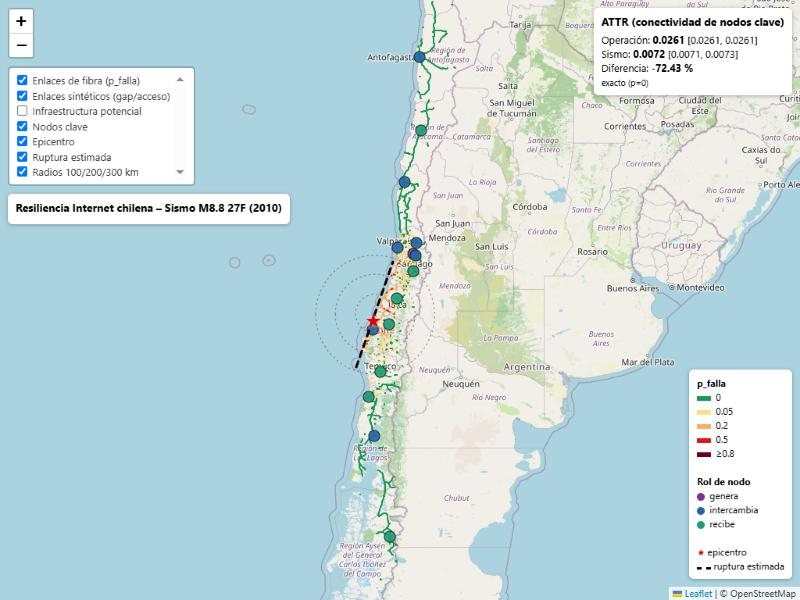
\includegraphics[width=0.85\textwidth]{../docs/mapa_general.jpg}
\caption{Vista general del mapa.}
\end{figure}

\begin{figure}[h]
\centering
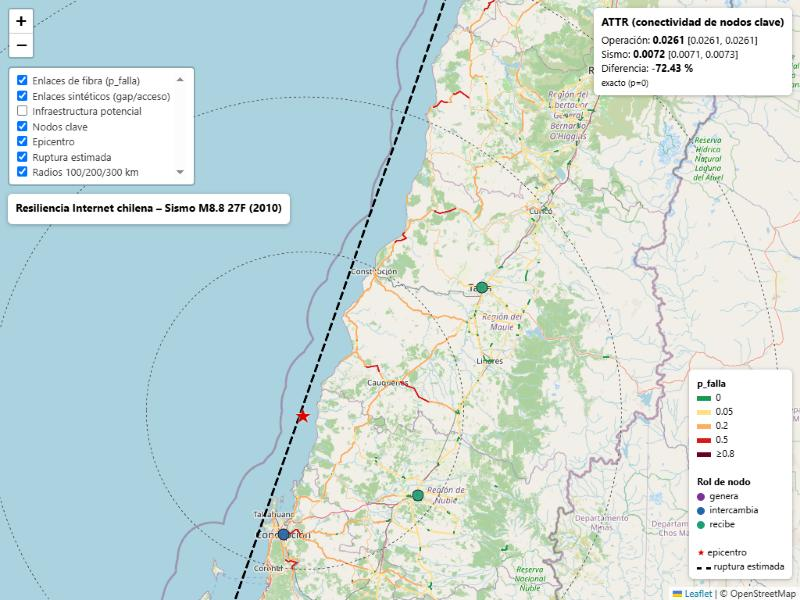
\includegraphics[width=0.85\textwidth]{../docs/mapa_zona_epicentro.jpg}
\caption{Zona del epicentro: enlaces con mayor probabilidad de falla en el Maule y el Biobío.}
\end{figure}

\clearpage
%=====================================================================
\section{Conclusiones}
%=====================================================================
La fibra óptica interurbana levantada por el Estudio (10\,313 km) no forma una red conexa: se
divide en 126 componentes y la mayor reúne sólo el 16,2\,\% de los vértices, en línea con el 17,1\,\%
que reporta el propio Estudio. Por eso el ATTR entre los 18 nodos clave es bajo incluso en operación
(0,0261): sólo 4 de los 153 pares están conectados, Santiago con La Serena y Concepción con Chillán.
Esta cifra no describe la Internet que usan las personas, sino la parte de la red física que se puede
verificar, y deja en evidencia cuánto depende la conectividad del país de tramos que no aparecen en
los datos públicos.

El terremoto M8.8, modelado con la atenuación de Youngs et al. (1997) y la tasa de roturas de Hazus,
reduce el ATTR a 0,0072, una caída del 72\,\%. El daño se concentra en el Gran Concepción, Arauco,
Ñuble y Maule, las mismas zonas donde el 27F cortó fibras en puentes colapsados, y el par
Concepción--Chillán queda prácticamente desconectado. El eje Santiago--La Serena también cae a cerca
del 11\,\%, no por la intensidad del sismo en el norte, sino porque la ruta no tiene alternativas y
la probabilidad de corte se acumula a lo largo de cientos de kilómetros en serie.

La lección principal coincide con las recomendaciones del Estudio: la vulnerabilidad de la red chilena
no viene sólo de la intensidad del sismo, sino de su forma. Una red troncal lineal y con forma de
árbol, sin rutas paralelas ni anillos, convierte cualquier corte en una desconexión. Agregar
redundancia geográfica (rutas alternativas, anillos regionales y el uso de cables submarinos como
respaldo de la troncal terrestre) tendría más efecto sobre el ATTR que reforzar tramos individuales.
El modelo tiene limitaciones importantes (fallas independientes, intensidad en roca, fibra aérea
tratada como enterrada y ausencia de fallas de nodos y energía, que fueron las que dominaron el 27F en
Santiago), pero el resultado es robusto a la principal decisión de modelación, el umbral de los enlaces
sintéticos.

%=====================================================================
\section*{Referencias}
\addcontentsline{toc}{section}{Referencias}
%=====================================================================
\begin{itemize}
\item NIC Chile Research Labs / SUBTEL (2019). \emph{Estudio y Recomendaciones sobre la Resiliencia de
la infraestructura de la Internet chilena}, proyecto CORFO 15BPE-47225. Respuesta SAIP AN002T0005610.
\item Neumayer, S., y Modiano, E. (2010). Network reliability with geographically correlated failures.
\emph{IEEE INFOCOM}.
\item Neumayer, S., Zussman, G., Cohen, R., y Modiano, E. (2011). Assessing the vulnerability of the
fiber infrastructure to disasters. \emph{IEEE/ACM Transactions on Networking}, 19(6).
\item Youngs, R. R., Chiou, S.-J., Silva, W. J., y Humphrey, J. R. (1997). Strong ground motion
attenuation relationships for subduction zone earthquakes. \emph{Seismological Research Letters},
68(1), 58--73.
\item Wells, D. L., y Coppersmith, K. J. (1994). New empirical relationships among magnitude, rupture
length, rupture width, rupture area, and surface displacement. \emph{BSSA}, 84(4), 974--1002.
\item Newmark, N. M., y Hall, W. J. (1982). \emph{Earthquake Spectra and Design}. EERI.
\item O'Rourke, M. J., y Ayala, G. (1993). Pipeline damage due to wave propagation. \emph{Journal of
Geotechnical Engineering}, 119(9).
\item FEMA (2024). \emph{Hazus Earthquake Model Technical Manual}, v6.1, capítulo de sistemas de
servicios (\emph{Utility Systems}).
\item Boroschek, R., Contreras, V., Kwak, D. Y., y Stewart, J. P. (2012). Strong ground motion
attributes of the 2010 Mw 8.8 Maule, Chile, earthquake. \emph{Earthquake Spectra}, 28(S1).
\item USGS ComCat, evento usp000h7rf:
\url{https://earthquake.usgs.gov/earthquakes/eventpage/official20100227063411530_30}.
\end{itemize}

\section{Link al repositorio}
Repositorio de la tarea: \url{https://github.com/TheRamdomX/Tarea-2-Ruteo}.

\end{document}
